% This is "sig-alternate.tex" V2.1 April 2013
% This file should be compiled with V2.5 of "sig-alternate.cls" May 2012
%
% This example file demonstrates the use of the 'sig-alternate.cls'
% V2.5 LaTeX2e document class file. It is for those submitting
% articles to ACM Conference Proceedings WHO DO NOT WISH TO
% STRICTLY ADHERE TO THE SIGS (PUBS-BOARD-ENDORSED) STYLE.
% The 'sig-alternate.cls' file will produce a similar-looking,
% albeit, 'tighter' paper resulting in, invariably, fewer pages.
%
% ----------------------------------------------------------------------------------------------------------------
% This .tex file (and associated .cls V2.5) produces:
%       1) The Permission Statement
%       2) The Conference (location) Info information
%       3) The Copyright Line with ACM data
%       4) NO page numbers
%
% as against the acm_proc_article-sp.cls file which
% DOES NOT produce 1) thru' 3) above.
%
% Using 'sig-alternate.cls' you have control, however, from within
% the source .tex file, over both the CopyrightYear
% (defaulted to 200X) and the ACM Copyright Data
% (defaulted to X-XXXXX-XX-X/XX/XX).
% e.g.
% \CopyrightYear{2007} will cause 2007 to appear in the copyright line.
% \crdata{0-12345-67-8/90/12} will cause 0-12345-67-8/90/12 to appear in the copyright line.
%
% ---------------------------------------------------------------------------------------------------------------
% This .tex source is an example which *does* use
% the .bib file (from which the .bbl file % is produced).
% REMEMBER HOWEVER: After having produced the .bbl file,
% and prior to final submission, you *NEED* to 'insert'
% your .bbl file into your source .tex file so as to provide
% ONE 'self-contained' source file.
%
% ================= IF YOU HAVE QUESTIONS =======================
% Questions regarding the SIGS styles, SIGS policies and
% procedures, Conferences etc. should be sent to
% Adrienne Griscti (griscti@acm.org)
%
% Technical questions _only_ to
% Gerald Murray (murray@hq.acm.org)
% ===============================================================
%
% For tracking purposes - this is V2.0 - May 2012

\documentclass{sig-alternate-05-2015}


\begin{document}

% Copyright
\setcopyright{acmcopyright}
%\setcopyright{acmlicensed}
%\setcopyright{rightsretained}
%\setcopyright{usgov}
%\setcopyright{usgovmixed}
%\setcopyright{cagov}
%\setcopyright{cagovmixed}


% DOI
\doi{10.475/123_4}

% ISBN
\isbn{123-4567-24-567/08/06}

%Conference
\conferenceinfo{PLDI '13}{June 16--19, 2013, Seattle, WA, USA}

\acmPrice{\$15.00}

%
% --- Author Metadata here ---
\conferenceinfo{WOODSTOCK}{'97 El Paso, Texas USA}
%\CopyrightYear{2007} % Allows default copyright year (20XX) to be over-ridden - IF NEED BE.
%\crdata{0-12345-67-8/90/01}  % Allows default copyright data (0-89791-88-6/97/05) to be over-ridden - IF NEED BE.
% --- End of Author Metadata ---

\title{Will I Get in? - Modeling the Graduate Admission Process for American Universities}
\subtitle{}
%
% You need the command \numberofauthors to handle the 'placement
% and alignment' of the authors beneath the title.
%
% For aesthetic reasons, we recommend 'three authors at a time'
% i.e. three 'name/affiliation blocks' be placed beneath the title.
%
% NOTE: You are NOT restricted in how many 'rows' of
% "name/affiliations" may appear. We just ask that you restrict
% the number of 'columns' to three.
%
% Because of the available 'opening page real-estate'
% we ask you to refrain from putting more than six authors
% (two rows with three columns) beneath the article title.
% More than six makes the first-page appear very cluttered indeed.
%
% Use the \alignauthor commands to handle the names
% and affiliations for an 'aesthetic maximum' of six authors.
% Add names, affiliations, addresses for
% the seventh etc. author(s) as the argument for the
% \additionalauthors command.
% These 'additional authors' will be output/set for you
% without further effort on your part as the last section in
% the body of your article BEFORE References or any Appendices.

\numberofauthors{3} %  in this sample file, there are a *total*
% of EIGHT authors. SIX appear on the 'first-page' (for formatting
% reasons) and the remaining two appear in the \additionalauthors section.
%
\author{
% 1st. author
\alignauthor
Narender Gupta\\
       \affaddr{University of Illinois at Urbana-Champaign}\\
       \email{ngupta18@illinois.edu}
% 2nd. author
\alignauthor
Aman Sawhney\\
       \affaddr{University of New Mexico}\\
       \email{asawhney@unm.edu}
% 3rd. author
\alignauthor Dan Roth\\
       \affaddr{University of Illinois at Urbana-Champaign}\\
       \email{danr@illinois.edu}
}
% There's nothing stopping you putting the seventh, eighth, etc.
% author on the opening page (as the 'third row') but we ask,
% for aesthetic reasons that you place these 'additional authors'
% in the \additional authors block, viz.
% Just remember to make sure that the TOTAL number of authors
% is the number that will appear on the first page PLUS the
% number that will appear in the \additionalauthors section.

\maketitle
\begin{abstract}
We study the graduate admission process in American universities. Our goal is to build a decision support model that provides candidates with pertinent information as well as the ability to assess their choices during the application process. This model is driven by extensive machine learning based analysis of large amounts of historic data available on the web. Our analysis considers factors including, but not limited to, standardized test scores and GPA as well as world knowledge regarding university \textit{reputation} and \textit{similarity} with other universities. The learning problem is modeled as a binary classification problem with latent variables that account for unavailable information, such as multiple graduate programs within the same institution.

An additional contribution of this paper is the creation of a new dataset of more than 25,000 student application data, covering hundreds of universities over several years. This dataset allows us to develop models that provide insight into student application behavior and university decision patterns. Our experimental study reveals some key factors in the decision process of programs and, consequently, allows us to propose a recommendation algorithm that provides applicants the ability to make an informed decision of programs to apply to given their profile, with high confidence of being accepted.
\end{abstract}


%
% The code below should be generated by the tool at
% http://dl.acm.org/ccs.cfm
% Please copy and paste the code instead of the example below. 
%
\begin{CCSXML}
<ccs2012>
<concept>
<concept_id>10002951.10003227.10003241</concept_id>
<concept_desc>Information systems~Decision support systems</concept_desc>
<concept_significance>500</concept_significance>
</concept>
<concept>
<concept_id>10002951.10003227.10003351</concept_id>
<concept_desc>Information systems~Data mining</concept_desc>
<concept_significance>300</concept_significance>
</concept>
<concept>
<concept_id>10010147.10010257</concept_id>
<concept_desc>Computing methodologies~Machine learning</concept_desc>
<concept_significance>500</concept_significance>
</concept>
</ccs2012>
\end{CCSXML}

\ccsdesc[500]{Information systems~Decision support systems}
\ccsdesc[300]{Information systems~Data mining}
\ccsdesc[500]{Computing methodologies~Machine learning}

%
% End generated code
%

%
%  Use this command to print the description
%
\printccsdesc

% We no longer use \terms command
%\terms{Theory}

\keywords{Graduate Admissions, Decision Support, Learning Model, Latent Variables, Recommendations}

\section{Introduction}
\label{sec:intro}
Every year, thousands of students apply to American graduate programs and in the process, discover that there is a dearth of reliable sources to aid them in making an informed decision. There are several sources that provide admission related statistics in aggregate form, but not tailored to individual profiles, thus, leaving the applicant with the only option of guessing and hoping for the best. Even though learning models have been used in variety of real-world applications, there is surprisingly little literature available on understanding admission dynamics and decision making.

A typical university application process involves the applicant submitting his transcripts, standardized test scores, a few letters of recommendation, a statement of purpose that expresses his aims, ambitions and research interests, and descriptive answers to a few additional questions. Test scores include GRE\footnote{Graduate Record Examination \tiny{www.ets.org/gre}}, language test scores - such as TOEFL\footnote{Test Of English as Foreign Language \tiny{www.ets.org/toefl}} or IELTS\footnote{International English Language Testing System \tiny{www.ielts.org}} etc. Since requirements, deadlines and the specific process to meet them is university specific, the applicant needs to first choose the universities he would apply to. Hence, an applicant is generally advised to start about an year in advance of the university deadlines to timely complete these requirements.

Given the uncertainty, a naive solution is to apply to a large number of universities. But, more applications imply a deeper investment of time and energy on the applicant's part. This also implies a greater monetary investment, which is a major concern for applicants from developing countries. An efficient strategy to circumvent this is to categorize the universities so that one can cover a wide spectrum by applying to a few representatives from each category. A popular scheme includes three categories: \textit{Ambitious}: where the chances of admission are slim; \textit{Reachable}: where the chances of admission are decent; \textit{Safe}: where there is a fair certainty of being accepted. Multiple admission offers resulting from these decisions allow the applicant to choose, suboptimally, their best option.

The description of these categories is very subjective, and even more subjective is the applicant's ability to predict his probability of \textit{Admit} i.e. chances of being admitted to a given program and, hence, the university categorization. This prediction is generally based on hearsay or semi-informed opinions, resulting in confusion and a waste of resources for both the applicant as well as the university. 

In this paper, we address this problem by developing a machine learning approach which enables applicants to make informed decisions by evaluating their chances of admission. We suggest a latent variable based generative modeling approach which is easily extensible. Another contribution of this paper is the dataset we provide which enables others to build upon the system we have created. Additionally, we analyze our system from student's perspective but it can be easily extended to university's perspective as well.

Some researchers have briefly reflected on the process of decision making, but only qualitatively \cite{dagap}.The work done by Waters et al. models the problem from the university's perspective \cite{waters:iaai13}. They used a learning approach to aid the university admission committee by identifying the candidates that are unlikely to be offered admission. Their model is quite simplistic, considering the problem as a straightforward classification problem (via Logistic Regression) without attempting to reveal the diverse and rich patterns in the data. More importantly, their approach is university centric and does not provide any support to the decision process of applicants. The primary reason for the lack of such endeavours is the unavailability of a relevant dataset. One contribution of our work is the creation of such a dataset, which we will make available to the community. The dataset allowed us not only to determine the acceptability of an application but also suggest better choices.

Works such as Bruggink et al. and Moore et al. utilize domain knowledge to build statistical models\cite{bruggink, moore}. Bruggink et al. model undergraduate university admissions to a private liberal arts college \cite{bruggink}. The model treats application components as independent variables 	and assumes the decision to be dependent (\textit{Admit} or \textit{Reject}) on these. The independent variables include GPA \footnote{Grade Points Average}, SAT scores, other academic scores and extracurricular factors all of which have been quantized. Beyond strong statistical assumption, this approach assumes that the modelled university (and its application pool) provide a good representation of the whole distribution. Our study shows that this is not the case because different universities focus on different features, and hence produce decisions differently. We conclude that learning a decision model should be done separately for each university, if possible. Moore et al. model the problem with rule induction using ID3 algorithm \cite{moore}. Such an approach without care for bounded depth is prone to overfitting. Similar to Bruggink et al. the model is centered around one university and considers very small applicant sample size \cite{bruggink}.


\section{Problem Modeling}
\label{sec:problem-modeling}

\subsection{Data}
\label{subsec:dataset}
\label{subsec:dataset}
There are several online resources where applicants share their admission experiences; Edulix is one commonly used resource \cite{edulix}. It is an active resource which hosts applicant profiles from all over the world. GRE scores, undergraduate university name, GPA, TOEFL scores and other accomplishments such as work experience and research publications pertinent to the graduate admissions are reported in the profile. In addition, users mention the universities that they applied to and the result of each application (\textit{Admit}, \textit{Reject} or \textit{Result Not Available}).

We collected the data present on this website. Since the data is self reported, it had some erroneous reports, which we identified and removed by completely deleting any such record. We also excluded any application that was not classified as either \textit{Admit} or \textit{Reject}. We observed that GRE and TOEFL scores have undergone various changes in grading scale over the years. Also, undergraduate institutions all over the world follow different scales for reporting GPA. As a standardization measure, we mapped these fields linearly to a scale of 0-100. An undergraduate university might be referred to by the differing names due to reasons such as usage of a popular acronym or spelling errors. We mitigated this problem by mapping the university names to their unique website URL.

In this paper we focus on modeling admission to computer science graduate programs, which form the plurality of our data. Our experiments are conducted only on this subset of the data. A few of the features of the resulting dataset for the computer science applications are in Table \ref{tab:dataset}.

\begin{table}[]
\centering
\caption{Features of Data}
\label{tab:dataset}
\begin{tabular}{ll}
& \\
\textbf{General Features} & \\
\hline
Total number of users before sanitization & 36,207 \\
Total number of users after sanitization & 26,148 \\
& \\
\textbf{Features for CS related dataset} & \\
\hline
Number of users & 10,788 \\
Application year range & [2001 2015] \\
Median Application Year & 2013 \\
Most Frequent Application Term & Fall \\
Number of universities with reported data & 313 \\
Number of applications per student (Mean) & 6 \\
Number of applications per university (Mean) & 51 \\
Number of undergraduate universities & 2353 \\
Degrees sought & [MS, PhD] \\
\hline
\end{tabular}
\end{table}


\subsection{Supervised Learning}
\label{subsec:supervised-learning}
Each university offers binary decisions to applicants (\textit{Admit} or \textit{Reject}) and this decision is unaffected by the decision of other universities. Hence, the overall problem can be modeled as a set of individual binary classification problems. Supervised learning algorithms can be trained using features extracted from a labeled dataset and evaluated on prediction accuracy. However, accuracy, in this case, is a biased metric since most universities have very low acceptance rates, some of them being as low as 5\%. In such a scenario, even by blindly rejecting all the applications the classifier will still evaluate to over 90\% accuracy, without the need to learn anything. Also, acceptance rates vary across universities and thus accuracy will not be a true representative of the learning model's performance. Hence, we chose F1 as our evaluation metric which combines precision and recall. Since number of admitted students is less than that of the rejected ones, we report our results for \textit{Admit} label which provides a stricter bound on evaluations. F1 score takes into account not just the correct number of predictions made for \textit{Admit} (\textit{Precision}), but also the ratio of \textit{Admit} students out of true \textit{Admit} count (\textit{Recall}).

$$F1 = \frac{2 \times Precision \times Recall}{Precision + Recall}$$
$$Precision = \frac{TP}{TP + FP}$$
$$Recall = \frac{TP}{TP + FN}$$

\begin{table}[]
\centering
\caption{Classification Context}
\label{tab:classification-context}
\begin{tabular}{|l|r|r|r|}
\hline
                  &  & \multicolumn{2}{r|}{True Condition} \\ \hline
                  &  &  Admit         & Reject          \\ \hline
\multirow{2}{*}{Predicted Condition} & Admit &  TP         & FP          \\ \cline{2-4} 
                  & Reject & FN          & TN          \\ \hline
\end{tabular}
\end{table}

\textbf{Feature Engineering:}
The dataset contains several fields such as standardized test scores and academic history records. We extract several numerical features from these such as GRE test scores (AWA\footnote{Analytical Writing Analysis}, Verbal \& Quantitative), undergraduate GPA, language test scores (TOEFL), as well as categorical features such as program applied to (e.g. MS, PhD), term (e.g. Fall, Spring) etc. These features are used for learning Logistic Regression, Support Vector Machine and Random Forest. Since most work available in the literature is confined to approaches we have mentioned so far, we`ll regard it as the baseline for any novelties that we propose.

\textbf{Ensemble Learning:}
To improve the system performance, we use ensemble learning. Training decision trees without bounded depth is prone to overfitting. But we can hope to generalize better if we use several limited-depth decision trees using partial data, and then feeding each decision as a feature into another regularized classifier. Constrained by the variance-bias trade-off, the second classifier captures variance of data through multiple underlying decision trees while keeping a limit on its own variance by choosing simple models such as linear separators e.g. soft-margin support vector machine. We create \textit{d} such limited-depth decision tree classifiers where each classifier is trained on a bootstrapped sample from the original dataset. Corresponding to decision of each such classifier, we get a feature for the next classifier. In section \ref{subsec:supervised-exp}, we perform grid search to find optimum value of \textit{d} for all universities.



\subsection{Generative Modeling}
\label{subsec:generative-modeling}
For a few universities, we noticed that our discriminative classifiers do not perform as expected, despite relatively large amount of data. we attribute it to the fact that some universities offer multiple degree programs that might target different kinds of applicants and have different admission criteria, e.g. professional master`s versus thesis master`s program at UIUC\footnote{University of Illinois at Urbana-Champaign}. Certain other universities, such as CMU\footnote{Carnegie Mellon University}, offer specific programs at same degree level such as master's degree in Machine Learning versus HCI\footnote{Human Computer Interaction} which fall under the purview of Computer Science. These distinctions, however, are not captured in the dataset, and are thus \textit{hidden} from our models. This distribution causes difficulties for linear separators which assume that data is coming from single source. In case the data is coming from multiple sources such as in Figure \ref{fig:linear}, it is impossible to linearly separate the data using a single classifier. To accommodate these phenomena, we use an \textit{Expectation-Maximization (EM)} algorithm that allows us to learn a model with a latent variable, capturing the missing information. The rest of this section, describes how we model the problem in this case. 

EM is one of the very effective techniques for finding a \textit{Maximum Likelihood Estimate} with \textit{hidden variables}. For the sake of brevity, we are not going into details of \textit{EM}. We will be using a setup similar to the one Grove et al. used in \cite{GroveRoth}.

We assume a hidden variable called Program Type, \textit{z}, which might carry assume multiple values. These values can hold different semantics based on university, e.g. different for UIUC and CMU, and, hence, we refer to them simply by the value assigned by the model to the hidden variable such as \textit{1, 2 ... k} etc. Once we learn the most likely model with the hidden variable \textit{z} taking \textit{k} values we can use it in two different ways.  In a soft-boundary setting, each student can be from either Program Type with some probability. In a hard boundary setting, the most likely cluster (program) completely owns the student record, and we can learn individual linear classifiers for each cluster. A student belongs to cluster $z=i$ if:
\begin{equation}P(student | z=i) > P(student | z=j), \forall {j\neq i}\end{equation}
where
\begin{equation}
\sum_j P(student | z=j) = 1
\end{equation}

We assume that an applicant \textit{belongs} to a program $ z \in \{1,2,...,k\} $ with probability $\alpha_r = p(z=r)$. Given this program, feature $x_i$ of the applicant $x$ is generated independently by a Gaussian distribution with model parameters $(\mu_i, \sigma_i)$.

Let us define a hidden variable, $ z \in \{1,2,...,k\} $. A student record (sample), \textit{x}, consists of \textit{(n+1)} features,
$$ x = (x_0, x_1, x_2, ..., x_n). $$
The likelihood of sample is given by
\begin{equation}
P(x) = \sum_z p(x | z) p(z)
\end{equation}
Incorporating each feature probability, the likelihood of the data sample can be expressed as:
\begin{equation}
P(x) = \sum_z \left( p(z) \prod_i p(x_i | z) \right)
\end{equation}

Starting with an initial set of parameters $\theta$, the probability that a data point $x^j = x^j = (x_0^j,x_1^j, ....x_n^j)$ comes from each of the $k$ values of $z$ is given by:

\begin{equation}
P^z_r = p(z=r | x^j) = \frac{p(z=r)\prod_i p(x^j_i | z=r)}{\sum_z \left(p(z)\prod_i p(x^j_i | z=r) \right)}
\end{equation}

Let $p^z_i = p(x_i | z=r)$, then we can compute the expected log-likelihood as follows:

\begin{align}
E(LL) &\equiv E\left(\sum_j \log P(x^j|\alpha_z , p^z_i) \right) \nonumber \\
&\equiv \sum_j E\left(\log P(x^j|\alpha_z , p^z_i) \right) \nonumber \\
&\equiv \sum_j \left( \sum_z P^j_z . \log P(z,x^j | \alpha_z, p^z_i)\right) \nonumber \\
&\equiv \sum_j \left( \sum_z P^j_z . \log (\alpha_z . \prod_i p(x^j_i | z))\right)
\end{align}

Assuming numerical features to be generated from a Gaussian distribution with parameters ($\mu, \sigma$), above equation can be expanded as:
\begin{align}
E &\equiv \sum_j \left( \sum_z P^j_z . \log \left( \alpha_z . \prod_i \frac{1}{\sigma^z_i \sqrt{2\pi}}\exp\left(-\frac{(x^j_i - \mu^z_i)^2}{2(\sigma^z_i)^2}\right)\right)\right) \nonumber \\
&\equiv \sum_j \left( \sum_z P^j_z . \left[ \log \alpha_z + \sum_i \left( -\log \sigma^z_i -\frac{(x^j_i - \mu^j_i)^2}{2(\sigma^z_i)^2} \right) \right]\right)
\label{eq:expected-ll}
\end{align}

Differentiating with respect to all parameters, we can find new values of $\alpha_z$, $\sigma^z_i$, and $\mu^z_i$, for which the expected (log) likelihood receives an extremal value. Since, $\alpha$ can only assume $k-1$ independent values because of $k$ states of $z$, we have:
\begin{equation}
\alpha_k = 1 - \sum_{i\in [1...k-1]}\alpha_i
\end{equation}

Using this equation and differentiating Eq (\ref{eq:expected-ll}) partially with respect to model parameters, we get following update rules:
\begin{equation}
\alpha_z = \Bigg\{
\begin{array}{ll}
	\alpha_k\frac{\sum_j P_z^j}{\sum_j P_k^j} & \mbox{if } z \neq k \\
	1 - \sum_{i\in [1...k-1]}\alpha_i & \mbox{if } z = k
\end{array}
\end{equation}
\begin{equation}
(\sigma^z_i)^2 = \frac{\sum_j \sum_z P^j_z (x_i^j - \mu^j_i)^2}{\sum_j \sum_z P^j_z}
\end{equation}
\begin{equation}
\mu^z_i = \frac{\sum_j \sum_z P^j_z x_i^j}{\sum_j \sum_z P^j_z}
\end{equation}

Using above update rules, and various initialization schemes, we performed multiple experiments with EM. Current results are reported for \textit{z}=2 in a hard-boundary setting.


\section{Experiments}
\label{sec:experiments}
Our experimental study is designed to investigate the following issues:
\begin{itemize}
\item The ability to to make reliable prediction on whether a specific student can be admitted to a given program.
\item Our ability to identify sub-programs in a given university, and its significance on the performance of our admission model. 
\item Understanding the factors that contribute to admission.
\item Understanding the differences among universities in terms of their admission decisions.
\end{itemize}
The rest of this section describes the details of our experimental study, and its results. For practical purposes, we selected a university for classification only if it has more than a certain number of applicant records. We chose the threshold of at least 10 admitted and at least 10 rejected students. In all our experiments we are reporting average F1 over 5-fold cross-validation.

\subsection{Discriminative Classifiers}
\label{subsec:supervised-exp}
We ran multiple experiments with various classifiers such as - SVM with linear kernel or Radial Basis Function kernel, Logistic Regression, Adaboost with decision trees, and Random Forest. We also experimented with all of the above classifiers by adjusting class weights according to sample frequency. Each of these setups is used in two different settings:
\begin{itemize}
\item Using simple features extracted from student records
\item Training \textit{d} decision tree classifiers with bounded-depth (depth=3) and then using predictions of these classifiers as features. Each decision tree is trained on 50\% data, selected randomly.
\end{itemize}
Using grid search, we found that \textit{d}=60 yields maximum average F1 over all universities. These classifiers can provide the probability of the label as well which we utilize in Section \ref{sec:recommendations}. We observed that SVM with RBF kernel and Random Forest (with adjusted class weights) perform the best, hence we will report only their results for further experiments. These experiments were conducted using software implementation of Scikit-learn \cite{scikit-learn}.

\subsection{Feature Ablation}
\label{subsec:ablation-exp}
These experiments were aimed at understanding the value in each feature. We trained multiple classifiers using single features and evaluated their performances. Then we iteratively added more features to each of the classifiers and evaluated gain in performance. Each feature, when considered individually, is the only classifying parameter. We call its corresponding F1 result the Discriminative Power of feature. It was observed that undergraduate GPA has the highest discriminative power and has an average F1 over all universities close to 0.65. Figure \ref{fig:ablation} shows how overall F1 increases if we sort the features into descending order of discriminative power and keep on adding them to the classifiers.


\subsection{EM}
\label{subsec:em-exp}
The EM model formulated in Section \ref{subsec:generative-modeling} was used to cluster students into different groups, representing potential programs. Subsequently, individual classifiers were learned for each of the clusters. Results for few of the universities for which significant growth was observed are listed in Table \ref{tab:em-gain}. As per the model assumption, EM bifurcates the data into two clusters (\textit{z}=2), each of which can be separated in a better way than the earlier cumulative cluster thereby increasing the performance of the models significantly. Improvement in F1 due to EM clustering is reported in Fig \ref{fig:simple_vs_tree_vs_em}.

\subsection{Understanding Institution Rankings}
\label{subsec:ranking-exp}
This experiment explored the role of \textit{reputation} or \textit{rank} of the applicant`s undergraduate institution in graduate admissions. Ranks could be categorical or numerically ordered. Each university may have a different view of how they perceive an undergraduate institution and, hence, rank it differently. But these ideas do not have a firm ground and the following experiments analyzed this hypothesis.

First, we investigated if the notion of an undergraduate institution`s rank or category even exists. If it does, providing this extra knowledge should help improve the classifier`s performance. Our dataset has applicant records from a variety of departments belonging to thousands of undergraduate institutions across many countries. Since it is not practical to rank all of them in numeric order, we used information from other proxies to group them into categories. These proxies included, but were not limited to, rankings provided by US News \cite{usnews}, QS (Top Universities) rankings \cite{qs}, Shanghai rankings \cite{shanghai}, and other lists provided by various government or non-government agencies such as 'List of Institute of National Importance in India' \cite{national-importance}.

Using these proxies, we created four categories:
\begin{itemize}
\item[A-] Institutions ranked as top tier and widely recognized.
\item[B-] Institutions ranked in the middle tier or recognized regionally.
\item[C-] Institutions ranked in the low tier.
\item[D-] Institutions that are neither recognized nor ranked.
\end{itemize}
We want to emphasize that our goal is not to come up with an \textit{`ideal'} university rank-list but to evaluate the existence of such a list. This can be answered by answering two sub-questions:
\begin{enumerate}
\item Does a list provide any gain in discriminative power of classifier?
\item Does any other list, similar or random, provide any gain in discriminative power of classifier?
\end{enumerate}

Our hypothesis was that if a largely agreed upon rank-list existed, and if our proxies are representative of such a list, then this rank-list should provide gain to the classifier. At the same time, any other list which deviates drastically from such a list should not provide comparable gain during classification.

This category distribution was referred to as \textbf{`Original Rank List' (ORL)}. ORL had following category distribution: A=47, B=217, C=363, D=2354. Next, we \textbf{consciously shuffled} this list using following rules:
\begin{enumerate}
\item A university can have either the same category as it originally had, or it can move to its closest category, e.g. B can move to either A or C. The probability of an institution moving to neighbor category is linearly proportional to the target size.
\item Each category still has the same number of institutions as it originally had.
\end{enumerate}

Since, we shuffled the institution categories based on precise rules, we called the result as \textbf{`Consciously Shuffled Rank List' (CSRL)}. We were taking into account that ranking of a university varies with ranking agencies or regions. In addition, we maintained the original category distribution (size of category) of the institutions. \textbf{`Randomly Shuffled Same Distribution Rank List' (RSSDRL)} was created by assigning a randomly chosen category to each institution but by maintaining original category distribution. Finally, we created a \textbf{`Randomly Shuffled Uniform Distribution Rank List' (RSUDRL)} by assigning a random category to each institution, without the constraint of maintaining original distribution. In RSUDRL, each category has uniform probability of occurring within the rank list. Results of these are shown in Fig \ref{fig:undergrad_rank_gain}.


\subsection{Impact of Change in Application Year}
\label{subsec:year-change-exp}
In this experiment, we asked the question - Do universities change taste of students over time? Hence, we explored the change in decision to an application in a different application year. Some assume that since there is an increment in the number of applications every year, admissions become more competitive over time. We performed a carefully controlled experiment to test the validity of this hypothesis. In this setting, for every university:
\begin{itemize}
\item[1.]Choose a training set (80\%) and test set (20\%), by random selection.
\item[2.]For each record in test set, record the application year, admission decision and prediction of classifier.
\item[3.]For each record in test set, change the application year (choose randomly between 2001 and 2015), and record the new prediction, using the classifier used in the previous step.
\item[4.]Perform this experiment for n(=100) iterations.
\end{itemize}
Our hypothesis was that if yearly factors do not have an effect then changing application year should not change the decision.


\subsection{Which Universities Go Together}
\label{subsec:similarity-exp}
One of the unique features of our dataset construction is that applicant records capture various university combinations that the users apply to along with their results. This allowed us to find patterns, and formulate similarities among universities. Apriori algorithm \cite{apriori} produces interesting results that are reported in table \ref{tab:apriori}. But Apriori favors heavily populated universities over the less frequent ones. Hence, we expanded our experiments to include null-invariant measures. We computed similarity of two universities based on candidate acceptance using several null-invariant measures such as: AllConf, Jaccard, Cosine Similarity, Kulczynski coefficient, MaxConf defined in \cite{Han2012243}.
Results of the experiments are reported in table \ref{tab:kulc} and \ref{tab:apriori}.\\\\\\


\section{Results}
\label{sec:results}

\subsection{Discriminative Classifiers}
\label{subsec:supervised-result}
\begin{figure}[t]
\centering
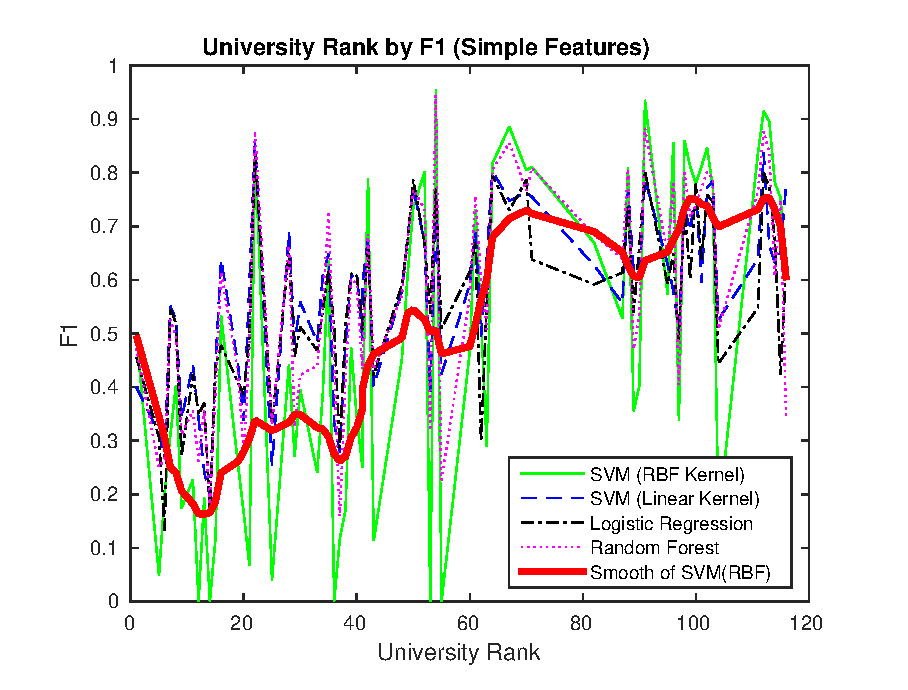
\includegraphics[scale=0.6]{simple_features.eps}
\caption{F1 scores for classification using supervised learning on simple features.}
\label{fig:simple_features}
\end{figure}

\begin{figure}
\centering
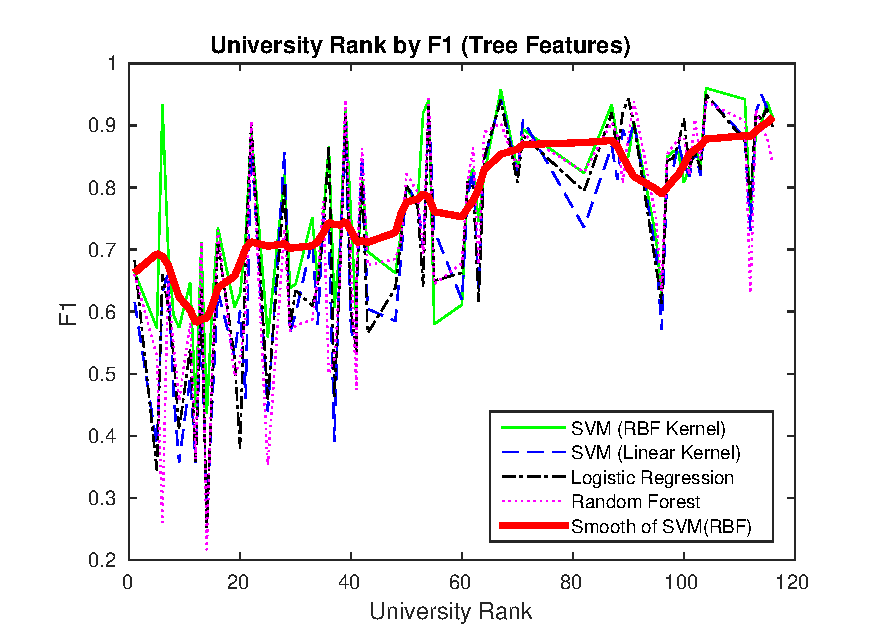
\includegraphics[scale=0.6]{tree_features.eps}
\caption{F1 scores for classification using supervised learning on bounded-depth decision tree features.}
\label{fig:tree_features}
\end{figure}

To garner insights out of classification results for different universities, we needed to sort them in some order. To explore the trends i.e. the variation in prediction performance on universities of varied reputation, an ordering on the basis of reputation was required. We chose this order to be US News Graduate School Ranking, primarily, because of its popularity among applicants. Whenever a rank was not available in this resource, a similar resource was consulted. In US News ranks, sometimes multiple adjacently ranked universities were stacked up on a single rank, and the resulting emptied out slots were left vacant. We flattened each stack to its nearest available slots. Fig \ref{fig:simple_features} shows F1 on y-axis and university ranking on x-axis.

These results are for 69 universities having more than a thresholded number of applicants. For simplicity purposes, we treated these discrete values as a continuous function while plotting the graph. It can be observed that SVM with RBF kernel yields best results, hence, a smooth curve, using moving averages of span 5, of it is also plotted for easy visualization. Similar graph is plotted for ensemble learning with Decision Tree features in Fig \ref{fig:tree_features}. Fig \ref{fig:simple_vs_tree} shows that Decision Tree feature classifier is a huge improvement over simple features.

\begin{figure}
\centering
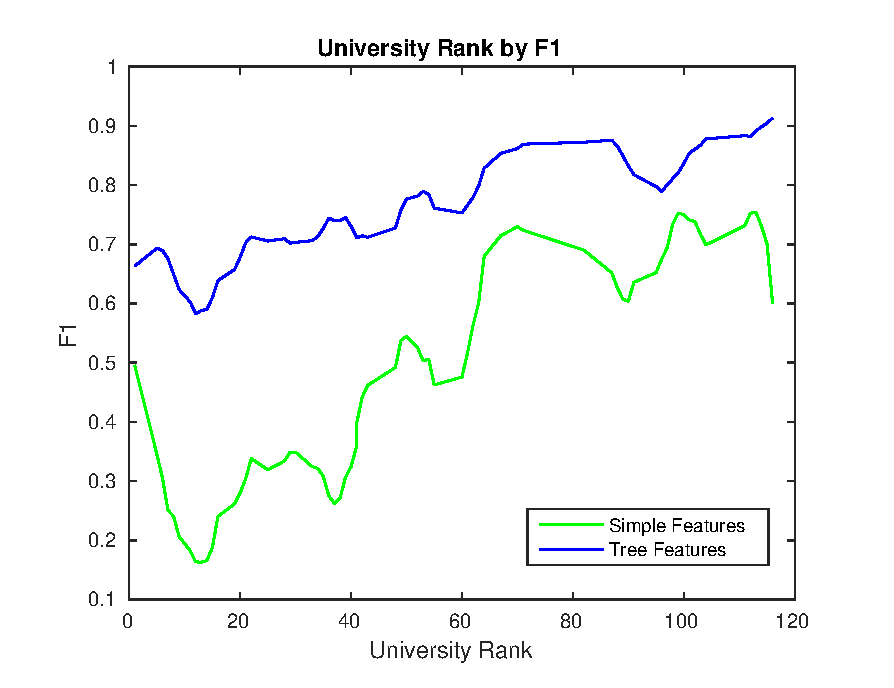
\includegraphics[scale=0.6]{simple_vs_tree.eps}
\caption{Comparison of Decision Tree feature classifier with baseline of simple feature classifier.}
\label{fig:simple_vs_tree}
\end{figure}

As we can see from Fig \ref{fig:tree_features} that we can get very good predictions for certain universities (F1 $\geq$ 0.8), while it is decent but not as good for certain others (0.6 $\leq$ F1 $<$ 0.8), and low for certain other universities. But it is interesting to see the growth trend in F1 as we go from top-tier to lower-tier rank universities. The trend represents that we can classify with very high confidence for lower-tier universities using available features, in spite of lack of qualitative features such as Statement of Purpose or Letter of Recommendation, Research Publications etc. At the same time, top-tier universities might put more focus on these qualitative features.\\

\subsection{Feature Ablation}
\label{subsec:ablation-result}
\begin{figure}[t]
\centering
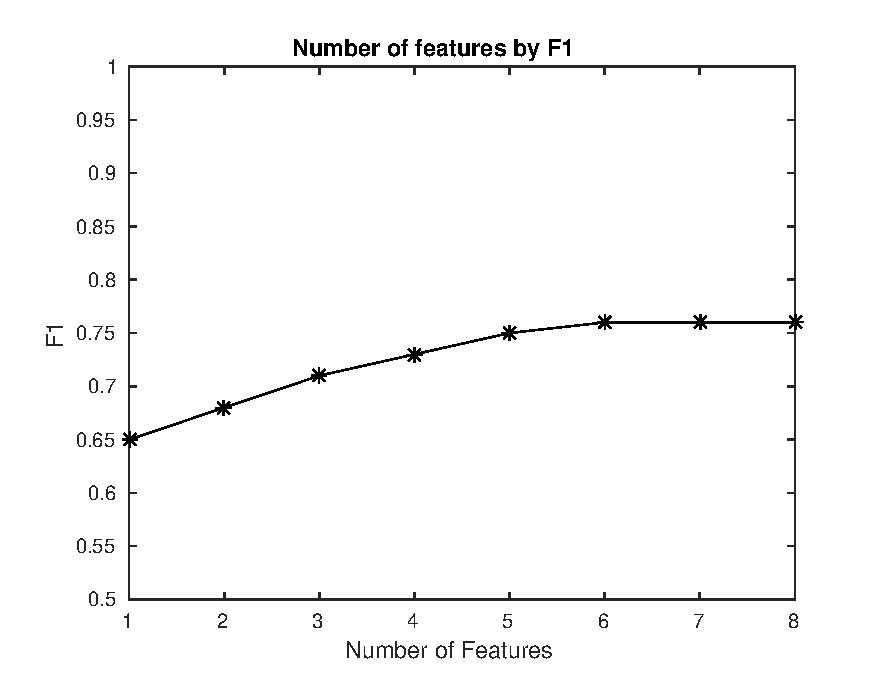
\includegraphics[scale=0.6]{ablation.eps}
\caption{Cumulative F1 as we keep on increasing features on top of GPA}
\label{fig:ablation}
\end{figure}

\begin{table}[t]
\centering
\caption{Discriminative Power of each feature}
\label{tab:ablation}
\begin{tabular}{p{0.5 cm} p{2.5 cm} p{1.3 cm} p{1.3 cm}}\\
Index & Feature Name & Cumulative F1 & Individual F1 \\ \hline
1 & GPA & 0.65 & 0.65 \\ \hline
2 & GRE Quant & 0.68 & 0.53 \\ \hline
3 & GRE Verbal & 0.71 & 0.58 \\ \hline
4 & GRE AWA & 0.73 & 0.45 \\ \hline
5 & TOEFL & 0.75 & 0.58 \\ \hline
6 & Program & 0.76 & 0.31 \\ \hline
7 & Term & 0.76 & 0.35 \\ \hline
8 & Previous Department & 0.76 & 0.42 \\ \hline
\end{tabular}
\end{table}

\begin{table}
\centering
\caption{F1 without each feature. Less F1 due to missing feature indicates more discriminative power of that feature.}
\label{tab:ablation-2}
\begin{tabular}{p{4.0 cm} p{1.3 cm}} \\
Ignored Feature Name & F1 \\ \hline
GPA & 0.7234 \\ \hline
GRE Quant & 0.7415 \\ \hline
GRE Verbal & 0.7422 \\ \hline
GRE AWA & 0.7491 \\ \hline
TOEFL & 0.7455 \\ \hline
Program & 0.7654 \\ \hline
Term & 0.7647 \\ \hline
Previous Department & 0.7518 \\ \hline
\end{tabular}
\end{table}

We observed from experiments that GPA results in a higher F1 score compared to any other single feature for any university. Also, if we calculate F1 by excluding individual features, exclusion of GPA causes maximum loss in F1. Both of these observations lead to the conclusion that GPA has the highest discriminative power among all available features. The result is intuitive as it validates the expectation that, broadly speaking, GPA is the prime factor in the admission process. It can also be seen that as the number of features that are considered is increased, performance goes up and is the highest when all the features are considered. Table \ref{tab:ablation} lists individual discriminative powers of each feature, as well as cumulative power for $i$ features i.e. when features ${1,...,i}$ are used for classification. Table \ref{tab:ablation-2} lists loss in F1 due to exclusion of each feature during classification. Fig \ref{fig:ablation} plots the cumulative discriminative power when we keep on adding features.


\subsection{EM}
\label{subsec:em-result}
\begin{figure}
\centering
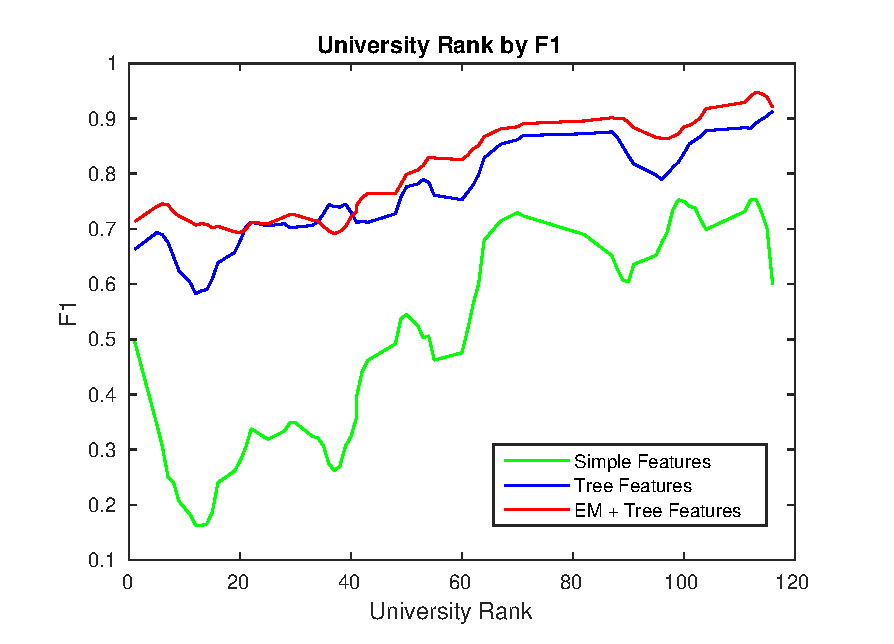
\includegraphics[scale=0.6]{simple_vs_tree_vs_em.eps}
\caption{Improvement in F1 scores due to EM clustering}
\label{fig:simple_vs_tree_vs_em}
\end{figure}

\begin{table}[t]
\centering
\caption{Gain in F1 score due to EM clustering}
\label{tab:em-gain}
\begin{tabular}{p{3.4 cm} p{0.8 cm} p{0.8 cm}| p{0.8 cm}}
\centering University & Tree & EM + Tree & EM Gain \\ \hline
UCSC\tablefootnote{University of California Santa Cruz} & 0.58 & 0.84 & 0.26 \\ \hline
SJSU\tablefootnote{San Jose State University} & 0.62 & 0.86 & 0.24 \\ \hline
UCLA\tablefootnote{University of California Los Angeles} & 0.45 & 0.68 & 0.23 \\ \hline
UMD\tablefootnote{University of Maryland College Park} & 0.43 & 0.66 & 0.22 \\ \hline
SUNY Binghamton\tablefootnote{State University of New York Binghamton} & 0.76 & 0.94 & 0.17 \\ \hline
UT Austin\tablefootnote{University of Texas Austin} & 0.57 & 0.74 & 0.17 \\ \hline
UC Boulder\tablefootnote{University of Colorado Boulder} & 0.80 & 0.94 & 0.14 \\ \hline
TAMU\tablefootnote{Texas A and M University College Station} & 0.75 & 0.86 & 0.11 \\ \hline
UIUC & 0.57 & 0.65 & 0.08 \\ \hline
CMU & 0.66 & 0.71 & 0.05 \\ \hline
\end{tabular}
\label{tab:em-gain}
\end{table}

Our model before the use of EM relied on the fact that data for each university is coming from a single source. The improvements in F1 as result of splitting the data according to EM formulation indicates that our model is able to capture underlying different distributions of source data. Also, since we know that UIUC offers different degree programs (Professional, Thesis), and CMU offers different specifications (Machine Learning, HCI etc) for the data reported as CS, it is probable that several other universities have more than one underlying distribution because of other factors. Fig \ref{fig:simple_vs_tree_vs_em} shows overall increase in F1 over all of the universities using EM splitting in two clusters (\textit{z}=2). Table \ref{tab:em-gain} reports significant improvement for some of the universities in our dataset by splitting data using EM.


\subsection{Undergraduate Institution Rankings}
\label{subsec:ranking-result}
\begin{figure}[t]
\centering
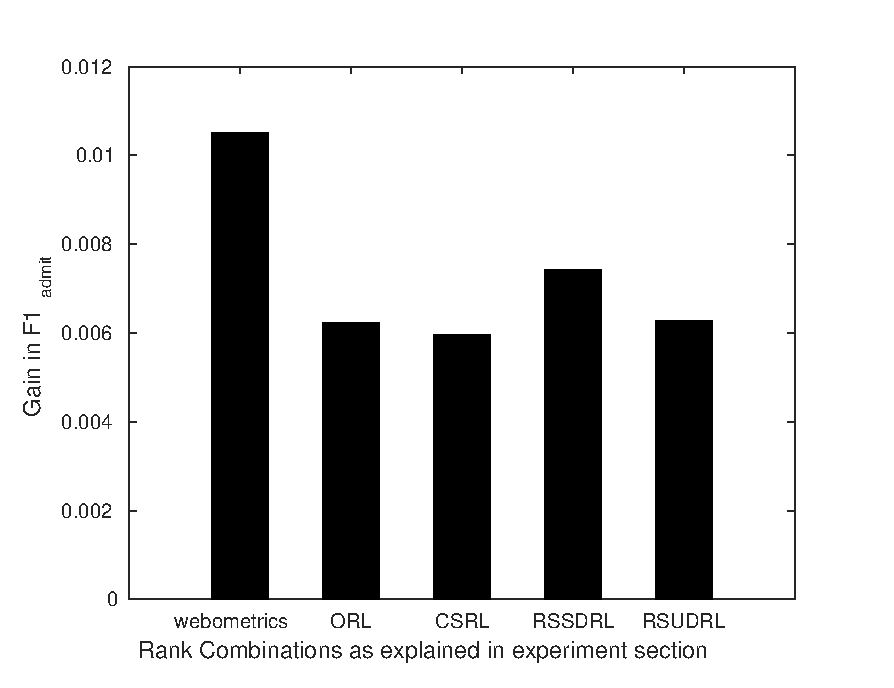
\includegraphics[scale=0.6]{undergrad_rank_gain.eps}
\caption{Gain in F1 due to various rank-lists}
\label{fig:undergrad_rank_gain}
\end{figure}

\begin{table}[]
\centering
\caption{Gain in F1 due to various rank-lists}
\label{tab:undergrad_rank_gain}
\begin{tabular}{p{2.5 cm} p{1.05 cm} p{1.05 cm} p{1.05 cm} p{1.05 cm}} \\
\centering University & ORL & CSRL & RSSDRL & RSUDRL \\ \hline
ASU\tablefootnote{Arizona State University} & \textcolor{red}{-0.0047} & \textcolor{red}{-0.1093} & \textcolor{red}{-0.1307} & \textcolor{red}{-0.2356} \\ CMU & \textcolor{red}{-0.0207} & \textcolor{red}{-0.7284} & \textcolor{red}{-0.0679} & \textcolor{red}{-0.2669} \\ \hline
Brown University & \textcolor{ForestGreen}{0.3856} & \textcolor{red}{-0.8298} & \textcolor{ForestGreen}{4.0007} & \textcolor{red}{-0.0333} \\
Purdue & \textcolor{red}{-2.4818} & \textcolor{red}{-1.4320} & \textcolor{red}{-1.2061} & \textcolor{ForestGreen}{0.5790} \\ \hline
UT Austin & \textcolor{ForestGreen}{5.7343} & \textcolor{ForestGreen}{4.1302} & \textcolor{ForestGreen}{3.5169} & \textcolor{ForestGreen}{5.2184} \\
Virginia Tech & \textcolor{ForestGreen}{4.0004} & \textcolor{ForestGreen}{5.4014} & \textcolor{ForestGreen}{5.7771} & \textcolor{ForestGreen}{4.5617} \\ \hline
\end{tabular}
\end{table}

Fig \ref{fig:undergrad_rank_gain} indicates that the addition of rank of the undergraduate institution feature led to the gain in performance. We evaluated the gain in terms of statistical significance over 100 iterations and it was significant with \textit{p-value < 0.0001}. This leads us to the conclusion that institution rank does play a role in the admission decision. Yet another interesting observation is that there is a comparable gain in all of the ways that we shuffled the rank-lists, consciously as well as randomly. This indicates that a popular rank-list provides only as much value as is provided by a random one.

Table \ref{tab:undergrad_rank_gain} provides gain in F1 corresponding to each rank-list for some of the universities. We see that the universities show three types of behavior:
\begin{enumerate}
\item There is loss in F1 for each of the rank-lists e.g. ASU or CMU
\item Some rank-lists provide gain while others cause loss in F1 e.g. Purdue or Brown universities.
\item There is gain in F1 for each of the rank-lists e.g. UT Austin or Virginia Tech
\end{enumerate}

A probable reason for this behavior (1) is that either the universities such as ASU or CMU don't use ranking system at all, and hence providing rank-lists causes the classifier to learn on irrelevant features causing a net loss, or none of the rank-lists is even close to the rank-lists used by these universities. For behavior (2), some of the rank-lists are close to the ones used by these universities while other rank-lists deviate drastically. For observation (3), all of the rank-lists are partially matching to the rank-lists used by these universities. Also, from $3^{rd}$ and $4^{th}$ rows in Table \ref{tab:undergrad_rank_gain}, it can be seen that one rank-lists provides gain to a specific university, while the other does the same for some other university.

Hence, it can be claimed that there is no single rank-list that every university uses, and there is no consensus over these ranks. So, two similar universities might respond differently to the same candidate even though all the other factors are consistent in his applications.



\subsection{Impact of Change in Application Year}
\label{subsec:year-change-result}
The experiment is aimed at testing the hypothesis that a change in the application year leads to a change in the decision. If an application was correctly classified initially then if there isn't any change in the competition of the application pool then it should still be correctly classified. Over 100 iterations, approximately 60K records were tested, out of which ~55K were classified correctly. It was observed that out of these, a vast majority (>98\%) retained the same label even after the change of application year.

We define competition per application to increase if increase in application year changed the decision from \textit{Admit} to \textit{Reject}, and vice versa. Out of all of the decision changes, a record was assigned `+1' if it showed that the competition increased, and `-1' if the competition decreased. Overall sum of these scores for most of the universities was very close to 0. For all of the universities, the overall sum was -56, which means 56/55K, approximately 0.1\% decrease in competition. Hence, it can be said that decision for an application depends solely on the university and the application, and not the application year.\\



\subsection{Which Universities Go Together}
\label{subsec:similarity-result}
As described earlier, applicants have the tendency to apply to universities in buckets \textit{(Ambitious, Reachable, Safe)}. This leads to the hypothesis that since applicants apply in buckets, it should be apparent through the similarity scores of the universities. As the results show this is infact the case. Kulczynski coefficient represents the average of conditional probability conditioned on each of the variables. Table \ref{tab:kulc} lists a few interesting associations based on the kulczynski coefficient and Table \ref{tab:apriori} lists such results for Apriori algorithm.

\begin{table}[htbp]
\caption{Interesting similar universities based on Kulczynski score}
\label{tab:kulc}
\begin {center}
\begin{tabular}{p{2.5 cm}| p{2.5 cm}| p{1.0 cm}}
\textbf{University 1} &\textbf{University 2} &\textbf{Kulc} \\ \hline
UChicago\tablefootnote{University of Chicago} & CSU\tablefootnote{Chicago State University} & 0.286 \\ \hline
UNCC\tablefootnote{University of North Carolina Charlotte} & UNLV\tablefootnote{University of Nevada Las Vegas} & 0.303 \\ \hline
CalTech\tablefootnote{California Institute of Technology} & UCR\tablefootnote{University of California Riverside} & 0.521\\ \hline
URI\tablefootnote{University of Rhode Island} & UWisc\tablefootnote{University of Wisconsin Madison} & 0.508 \\ \hline
\end{tabular}
\end {center}
\end{table}

\begin{table}[htbp]
\caption{Universities that go together based on Apriori algorithm}
\label{tab:apriori}
\begin {center}
\begin{tabular}{p{3 cm}| p{3 cm}| p{1 cm}}
\textbf{University 1} &\textbf{University 2} &\textbf{Support} \\ \hline
UM Twin\tablefootnote{University of Minnesota twin cities} & SUNY Stony\tablefootnote{State University of New York Stony Brook} & 218 \\ \hline
UIC\tablefootnote{University of Illinois Chicago} & Indiana\tablefootnote{Indiana University-Bloomington} & 112 \\ \hline
Cornell University & SUNY Stony & 97 \\ \hline
SUNY Buffalo\tablefootnote{State University of New York Buffalo} & GMU\tablefootnote{George Mason University} & 75 \\ \hline
\end{tabular}
\end {center}
\end{table}



\section{Recommendations}
\label{sec:recommendations}
Since, now we have a system that can predict application decisions for a university, we can utilize it  to aid students in making informed choices. In Section \ref{subsec:similarity-result}, we provide evidence that students apply to universities based on their notion of `Ambitious', `Reachable' and `Safe' buckets. We include this notion into our algorithm to generate recommendations. Since the classifier system we have is not 100\% accurate, it can generate erroneous recommendations if we simply classify for each university and return the results. Fig \ref{fig:simple_vs_tree_vs_em} shows that although the trend in university ranks is not strictly monotonous, it becomes very smooth if we cluster neighboring universities and then plot it. Hence, we cluster universities and employ multi-level classification to produce robust results while generating recommendations.

The first level of decision is coarse and the next level result is fine-grained. While classifying coarsely over a range of universities, we mix  the records of all universities inside a cluster and train a single classifier on all of them. If the universities in the cluster are similar, the classifier learns the common patterns of admission versus rejection and provides a more general decision than any of the component universities. While in Fine-grained classification an individual classifier is trained for each university.

This algorithm consists of 5 steps:
\begin {enumerate}
\item \textbf{University clustering}
	\begin {itemize}
	\item Cluster similar universities together based on US News rankings e.g. Universities in rank [1,10] fall into cluster 1, universities from [11,20] fall into cluster 2 and so on. 
	\end {itemize}
\item \textbf {Coarse classification}
	\begin {itemize}
	\item Using coarse decision, we find the cluster that offers \textit{Admit} and is closest to the top-tier universities. We call this cluster as `Reachable' because it is the best ranked university cluster that can offer Admission.
	\end {itemize}
\item \textbf {Reachable Universities}
	\begin {itemize}
	\item Perform fine-grained classification on each of the universities in `Reachable', and return those which produce an \textit{Admit} with highest probability.
	\end {itemize}
\item \textbf {Safe Universities}
	\begin {itemize}
	\item We call the cluster next to `Reachable' as `Safe' because it also offers admission and does so with higher probability. Then fine-grained classification is applied on `Safe' to report Safe universities.
	\end {itemize}
\item \textbf {Ambitious Universities}
	\begin {itemize}
	\item For `Ambitious' universities, we find those universities which are similar to the ones produced by `Reachable' and `Safe' but are towards the top tier universities and hence do not offer admission. These similar universities are based on the higher similarity score based on common admissions.
	\end {itemize}
\end {enumerate}

In step 1, the benefit of using US News rankings is that as the universities get closer to top rank, probability of admission of any candidate decreases. We also verified the same observation from data. As a future work, there many clustering schemes can be employed here, including university similarity scores reported in section \ref{subsec:similarity-result}, as long as proximity of various clusters is known.

\section{Conclusions}
\label{sec:conclusions}
This paper studies the graduate admission process in American universities using a machine learning approach. Our goal is to build a decision support model that allows candidates to make informed decisions on which schools to apply to, what are their chances of admission, and a slew of other decision-related issues. We modeled the decision process as a learning problem and presented a system that can achieve high accuracy and can be generalized across multiple universities. By employing many approaches towards solving this problem, such as supervised learning and generative modeling, we prove that a mixture of approaches can provide better results than any of the individual approaches. We also provide a dataset that provides avenues for further research. This work can be extended in multiple ways such as towards improving accuracy or validating common notions. Some of the additions of this work may include expanding the EM formulation by modeling further variables such as undergraduate institution ranking mechanism. We proved that every university has a custom ranking mechanism. This mechanism can be modeled as a distribution which can, then, be assigned to one of the hidden variables in the EM model. Theoretically, such a model has more expressive power and can, thus, learn better regarding application decisions. We believe this is but a brisk start to the research that can be performed on the topic. Many more enhancements are possible by expanding the dataset and extracting richer data features from Letters of Recommendation or Statement of Purpose. By asking these questions and providing this dataset, we hope to initiate a discussion that can lead to better understanding of how academia accepts its new members.


%
% The following two commands are all you need in the
% initial runs of your .tex file to
% produce the bibliography for the citations in your paper.
\bibliographystyle{abbrv}
\bibliography{Will_I_Get_In}  % sigproc.bib is the name of the Bibliography in this case
% You must have a proper ".bib" file
%  and remember to run:
% latex bibtex latex latex
% to resolve all references
%
% ACM needs 'a single self-contained file'!
%
% This next section command marks the start of
% Appendix B, and does not continue the present hierarchy
% That's all folks!
\end{document}
